\paragraph{} 
Let $n\times m$ be the size of the matrix. We call $c_i$ the integer sum of the column $i$ of the matrix, and $r_i$ the integer sum of the row $i$ of the matrix. We are going to show a way to compute a right rounding using max-flow algorithm.

\begin{figure}[h]
	\centering
		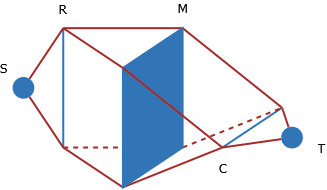
\includegraphics[width=10cm]{Diagramme1.png}
	\caption{Blue = Vertexes; Red = Edges}
	\label{fig:Diagramme1}
\end{figure}

\paragraph{}
We construct the following graph (see Fig. \ref{fig:Diagramme1}:
\paragraph{Vertexes}
\begin{itemize}
\item a source S
\item a sink T
\item n vertexes called $R_1,...,R_n$
\item m vertexes called $C_1,...,C_m$
\item n x m vertexes called $M_{1,1},...M_{n,m}$
\end{itemize}

\paragraph{Edges}
\begin{itemize}
\item n edges from S to $R_i$ with capacity $r_i$
\item m edges from $C_i$ to T with capacity $c_i$
\item n x m edges from $R_i$ to $M_{i,j}$ with capacity 1
\item n x m edges from $M_{i,j}$ to $C_j$ with capacity 1
\end{itemize}

\paragraph{}
Our graph is made so that the not-rounded matrix gives us a possible flow of capacity $r_1 + ... + r_n$ which is maximal because it saturates both the source and the sink. However, since every capacity of an edge of the graph is an integer, the solution given by the max-flow algorithm will have integer values. That means we get our rounding with the solution of max-flow algorithm.

\paragraph{}
Furthermore our algorithm is polynomial, because the size of the graph is a linear function of the size of the input matrix and Max-Flow is polynomial.